\graphicspath{{./assets/}}
\setcounter{mtc}{3}
\chapter{ 1st Sprint: Maintenance of existing resources  }
\fancyhead[R]{\ungaramond\small\textbf{Chapter III. 1st Sprint: Maintenance of existing resources }}
\minitoc
\newpage


\section*{Introduction}
The first sprint was dedicated towards exploring the existing services and resources, performing some minor changes and putting in place a backup strategy.

\section{Sprint backlog :}

\begin{longtable}[H]{|m{1.5cm}|m{3cm}|m{1.5cm}|m{8cm}|}
\hline
{\textbf{EpicID}} & {\textbf{Epic}} & {\textbf{StoryID}} & {\textbf{Story}} \\
\hline
1 &  \raggedright Exploring assets.	& 1.1  & SCM structuring: service components need to be split into different repos. \\
\cline{3-4}
& & 1.2 &  	Keeping track of developed applications and their requirements \\
\hline
2  & Maintenance. &	2.1	 &  Rebuilding optimized containers for developed applications. \\
\cline{3-4}
& & 2.2 & Backup of existing data on current infrastructure in S3 containers.\\
\hline
\caption{Table sprint Backlog}
\end{longtable}

\section{Maintenance operations}

In this sprint, we have assembled standalone self-hosted services into a single stack of upgraded container versions in order to provide better visibility of workloads. A container management platform was then added to this stack to improve on operability. 
The following figure is the deployment diagram of the resulting docker-compose stack:

 \begin{figure}[H] 
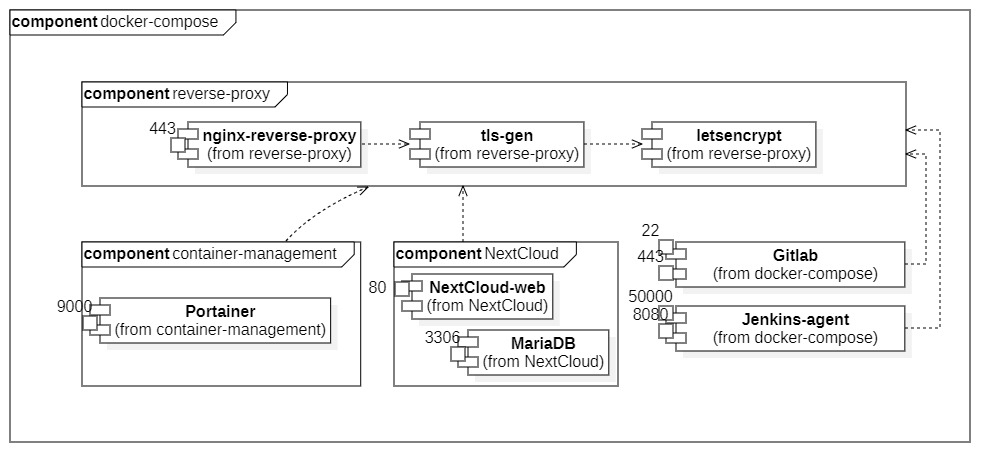
\includegraphics[width=1.0\textwidth,angle=00]{assets/f9.jpg}
\caption{PaaS infrastructure}
\label{fig:f9}
\end{figure}

\section{Application overview and SCM structuring.}

Two main applications were in development during this project. We have recommended a better source code management strategy that resulted in separating services into different repos in order to optimize the container image creation process. The resulting deployment diagram Is as follows:
 
\section*{Conclusion}
\paragraph{}In this chapter we have successfully performed

